\chapter{The smoothness assumption}
Going further with the spectral analysis, some other intuitions about the graph spectrum can be conveyed from the from the classical setting to the graph setting.

One of them is that in the classical setting the eigenvalues carry a specific notion of frequency: complex exponentials related to lower frequencies are relatively smooth, slowly oscillating functions whereas for high frequencies the associated complex exponentials oscillate more rapidly. Reporting this onto the graph spectral settings, we see that the Laplacian eigenfunctions associated with lower eigenvalues can be seen as smooth, while the ones related to higher eigenvalues tend to oscillate more intensively. \cite{Shuman2016} In the specific case of the null eigenvalue  the related eigenvector ($\chi_0$) is constant and equal to $\frac{1}{\sqrt{N}}$ \cite{Shuman2013}.

Taking a step back, one of the common simple assumptions about data residing on graphs, is that the signal changes smoothly between connected nodes; in this, a simple way to quantify how smooth is a set of vectors residing on a weighted undirected graph, is through the function:
\begin{equation}
\frac{1}{2} \sum_{i,j}W_{i,j}||\rchi_i - \rchi_j||^2
\label{eq:smooth}
\end{equation}
with $W_ij$ representing the weight between node $i$ and node $j$, as usual, and $\rchi_i$ and $\rchi_j$ representing two vectors in $\rchi_1,\rchi_2,\dots,\rchi_N \in \R$. This means that if two vectors $\rchi_i$ and $\rchi_j$ reside on two nodes connected by a high $W_{ij}$, then they are expected to have a small distance. \autoref{eq:smooth} can be thus rewritten in matrix form as \cite{Kalofolias2016} :
\begin{equation}
\tr(\rchi^T L \rchi)
\label{eq:smoothMatrix}
\end{equation} and, recalling that the Laplacian matrix can be expressed as:
\begin{equation}
L = \rchi \Lambda  \rchi
\label{eq:diag}
\end{equation}
with $\Lambda$ being the diagonal matrix containing the associated eigenvalues of the Laplacian, then we can insert \ref{eq:diag} in \ref{eq:smoothMatrix}, obtaining:
\begin{equation}
\tr(\rchi^T L \rchi) = \tr(\rchi^T \rchi \Lambda \rchi^T \rchi) = \tr(\Lambda)
\end{equation}
This result clearly explains the relation between the signal smoothness and the eigenvalues of the Laplacian that we presented at the beginning of the paragraph. \autoref{fig:osc} shows different graph Laplacian eigenvectors for a random graph. The eigenvectors associated to larger eigenvalues tend to oscillate more rapidly and to have dissimilar values on vertices connected by a high weight edge, this moreover bringing to higher occurrences of zero crossing associated to the graph Laplacian. \cite{Shuman2013}.

\begin{figure}
\centering
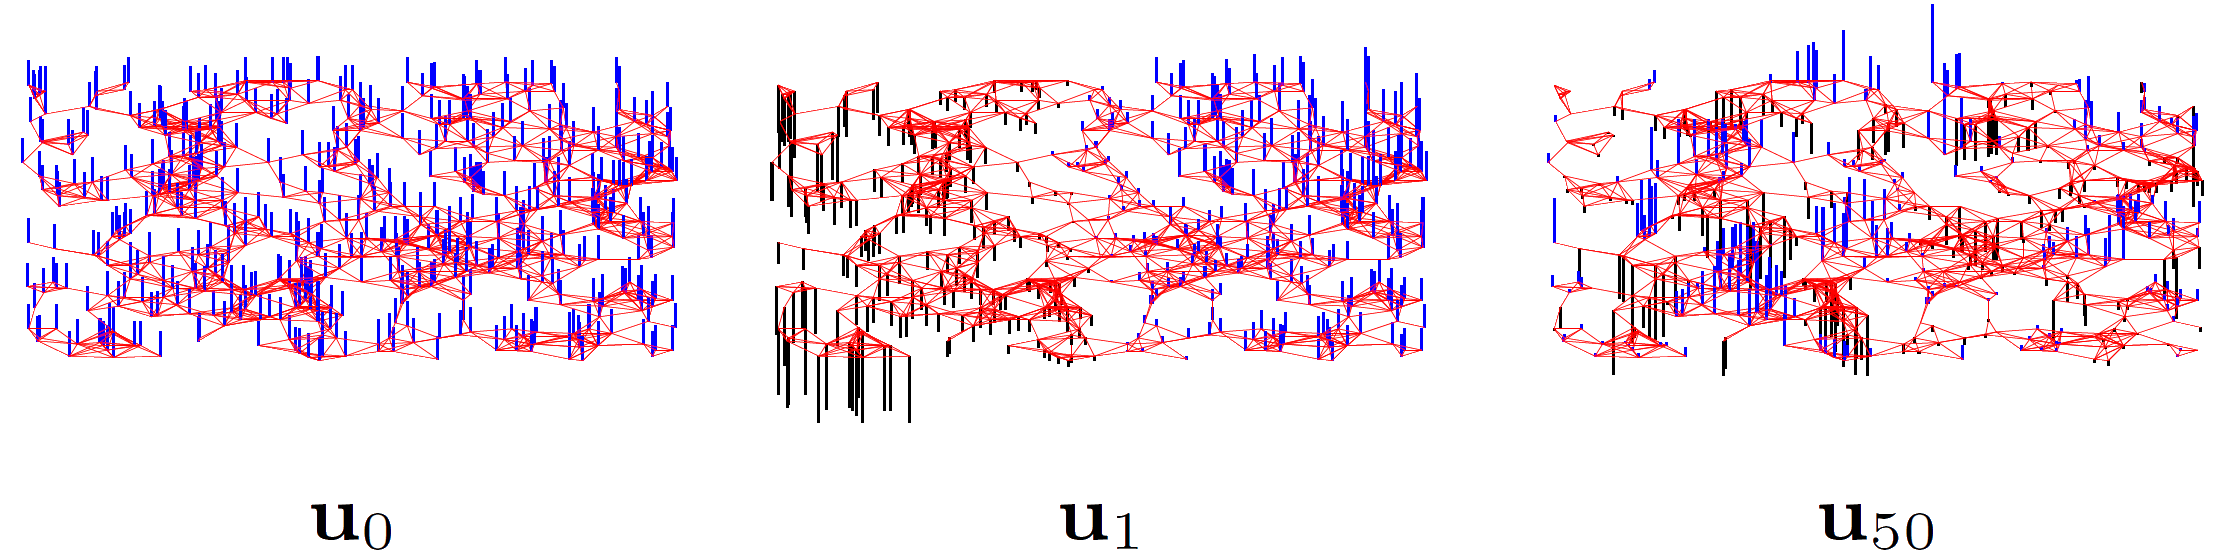
\includegraphics[width = .9\textwidth]{Oscillations.png}
\caption{three graph Laplacian eigenvectors for a random sensor network graph. It can be seen how $\chi_{50}$ contains definitely more zero crossing than the other two vectors $\chi_0$ and $\chi_1$}
\label{fig:osc}
\end{figure}

\section{Smoothness and sparsity}
In \cite{Kalofolias2016} the previous notion of smoothness is directly connected with the one of graph sparsity: in fact they show that the smoothness term can be seen equivalently as a weighted $l^1$ norm of the adjacency matrix, which being minimized can lead to a graph with a sparse set of edges, that prefers only the ones associated to small distances in the \textit{pairwise distances matrix} $\Z \in \R^{N\times N}_+$ defined as $\Z_{i,j} = ||\chi_i - \chi_j||^2$.

This concept is strictly connected with the compressibility property of a signal, since previous studies validate the hypothesis that smooth signals are likely to be compressible in the frequency domain. In \cite{Zhu2012} it has been shown that the liner approximation error is upper bounded by the overall variation of the signal, this bringing to the conclusion that if the total variation of a signal is small, then the approximation error is small. This resulting in the fact that the signal can be well approximated by a small portion of the Fourier coefficients.
